\chapter{性能评测}
\section{实验环境及方法}
我们在16台戴尔R720服务器上评估ClickNP的性能。每个FPGA都通过2个以太网端口与机架顶(top-of-rack, ToR)的戴尔S6000交换机相连。
我们在Windows Server 2012 R2上运行ClickNP。对于在Linux上运行的软件网络功能,我们使用CentOS 7.2平台,其内核版本为3.10。

为了测量网络功能的延迟,我们通过端口2将处理得到的包转发至回声(Echo)服务器。
回声服务器的FPGA中烧有回声逻辑,将收到的包发回其来源。
我们据此比较从端口1收到包起至从端口2收到回声包的时间差,得到精确到纳秒的延迟时长。
回声造成的延迟可以预先校正。

在我们的实验中,测试流量由包生成器PktGen产生,在包大小恒定为64字节时,
生成包的速率最高达到54.8Mpps。

\section{数据吞吐率及处理延迟评估}
\subsection{OpenFlow防火墙}
我们在实验中将OpenFlow防火墙与Linux防火墙以及Click+DPDK进行对比。
Linux防火墙采用IPSet处理精确匹配规则,采用IPTables处理模糊匹配规则。
我们在结果中引入了所使用的戴尔S6000交换机的性能作为参照,其防火墙处理能力有限,
只支持1.7K条模糊匹配规则。

值得一提的是,原先的Click+DPDK不支持接收端扩放(receive side scaling, RSS)。
我们在实验中修复了这一问题,而且发现Click+DPDK只需要4个核就可达到其最佳性能。
与此同时,对于Linux防火墙,我们需要尽可能地增加核数来提升其性能。
然而接收端扩放的限制使其最多只能使用8个核。

\begin{figure}[htbp]
\centering
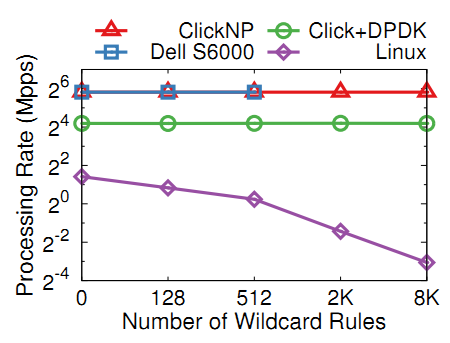
\includegraphics[width=4in]{ofwrate}
\caption{防火墙模糊匹配速率对比} \label{fig:ofwrate}
\note{包大小为64字节}
\end{figure}
图~\ref{fig:ofwrate} 展示各防火墙在不同数量模糊匹配规则下的处理速率对比。
可见ClickNP和S6000均可达到56.4Mpps的最大速率。

Click+DPDK的处理速率大约可达18Mpps。Click采用了静态决策树来实现模糊匹配,因而其处理速率不随规则增多而降低。
然而该决策树的实现需要基于所有规则的先验知识,在运行时更新规则很困难。

基于IPTable的Linux防火墙处理速率低达2.67Mpps。
而且因为IPTable的模糊匹配是线性的,所以其处理速率随着规则的增多呈倒数级下降。

\begin{figure}[htbp]
\centering
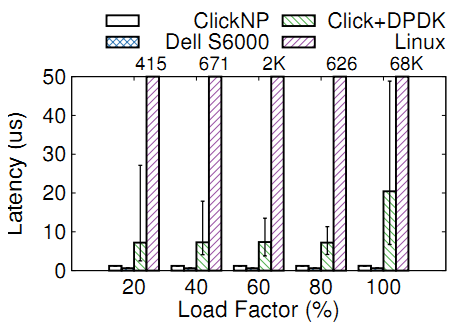
\includegraphics[width=4in]{ofwlatload}
\caption{不同负载下防火墙处理延迟对比} \label{fig:ofwlatload}
\note{包大小为64字节,误差杆置信水平为90\%}
\end{figure}
图~\ref{fig:ofwlatload} 展示各防火墙在不同负载下的小包处理延迟。
鉴于不同防火墙的处理能力差别明显,我们根据系统最大处理速率将负载标准化处理。
据图可见,在各个负载下,FPGA (ClickNP)和专用集成电路(S6000)的延迟均保持在2微秒以下,
相比之下软件处理的延迟大得多且不稳定,例如在高负载下Click+DPDK的延迟甚至高达50微秒。

\begin{figure}[htbp]
\centering
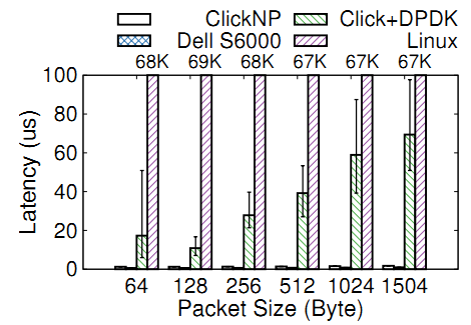
\includegraphics[width=4in]{ofwlatsize}
\caption{各防火墙处理不同大小包延迟对比} \label{fig:ofwlatsize}
\note{误差杆置信水平为90\%}
\end{figure}
图~\ref{fig:ofwlatsize} 展示面对不同大小的包时各防火墙的处理延迟。
据图可见,软件处理包的延迟随包的增大而增加,其主要原因是内存读取的增加。
相比之下,FPGA和专用集成电路的处理延迟不受包大小的影响。

在所有的测试中,ClickNP OpenFlow防火墙的CPU占用率都低于5\%。我们据此得出的结论是,
OpenFlow防火墙具有接近专用集成电路的处理性能,且更加灵活、易于重新配置。

\begin{figure}[htbp]
\centering
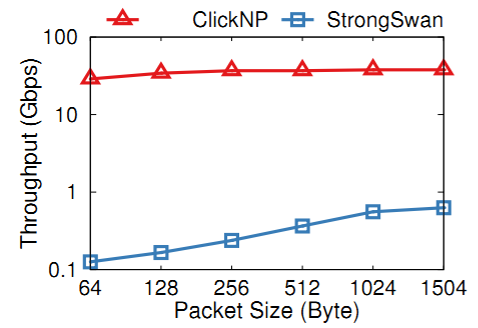
\includegraphics[width=4in]{ipsecrate}
\caption{互联网安全协议网关吞吐率对比} \label{fig:ipsecrate}
\end{figure}

\subsection{互联网安全协议网关}
我们将IPSecGW与strongSwan进行对比,采用AES-256-CTR算法加密及SHA-1算法认证。
图~\ref{fig:ipsecrate} 展示处理不同大小包的网关吞吐率对比。
据图可见,IPSecGW的吞吐率可以达到链路带宽,即在处理64字节包时达到28.8Gbps,
在处理1500字节包时达到37.8Gbps。相比之下,StrongSwan的最大吞吐率仅为628Mbps,
且随着包大小的减小而降低。这是因为需要处理的包数随着包大小的减小而增加,
因而系统需要计算更多SHA-1签名。

\begin{figure}[htbp]
\centering
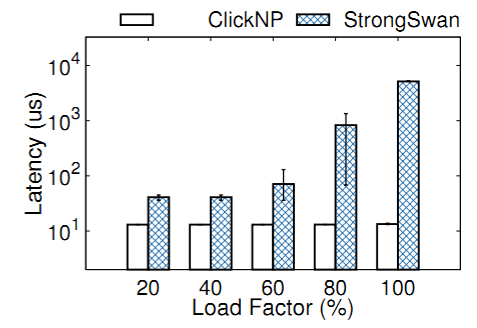
\includegraphics[width=4in]{ipseclat}
\caption{互联网安全协议网关延迟对比} \label{fig:ipseclat}
\note{误差杆置信水平为90\%}
\end{figure}
图~\ref{fig:ipseclat} 展示不同负载下的网关延迟对比。
据图可见,IPSecGW的延迟一直保持在13微秒以下,而StrongSwan的延迟更大且不稳定,最高甚至达到5毫秒。

\begin{figure}[htbp]
\centering
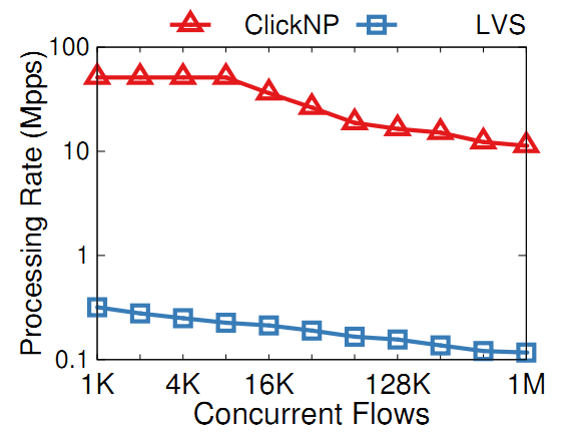
\includegraphics[width=4in]{l4rate}
\caption{第4层负载均衡吞吐率对比} \label{fig:l4rate}
\note{包大小为64字节}
\end{figure}

\subsection{第4层负载均衡}
我们将L4LB同Linux Virtual Server (LVS)进行对比。在压力测试中,我们向单个虚拟IP地址生成了大量并发的UDP流。
如图~\ref{fig:l4rate} 所示,当并发的流少于8K个时,L4LB吞吐率可以达到链路上限51.2Mpps。
但随着并发数进一步增加,吞吐率开始下降,这是L4LB流缓存缺失导致的。当遇到缓存缺失时,
L4LB需要访问一次DDR存储器,因而吞吐率下降到了11Mpps。相比之下,Linux Virtual Server在任何并发数下的吞吐率都很低,
这是因为LVS将同一虚拟IP地址的所有包均交给同一CPU核来处理,导致吞吐率被限制在200Kpps。

\begin{figure}[htbp]
\centering
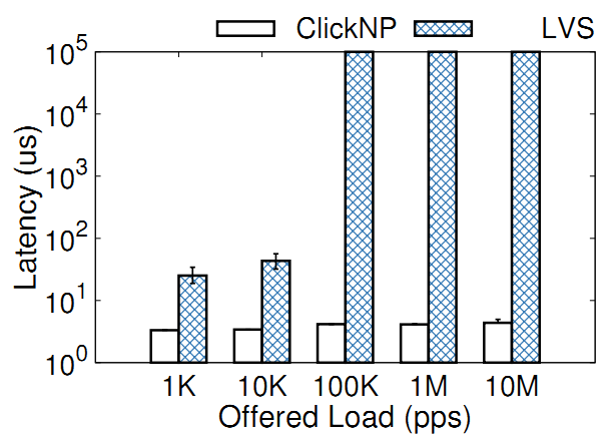
\includegraphics[width=4in]{l4lat}
\caption{第4层负载均衡延迟对比} \label{fig:l4lat}
\note{包大小为64字节,并发数为100万}
\end{figure}
图~\ref{fig:l4lat} 展示不同负载压力下的负载均衡延迟对比。
据图可见,在不高于10Mpps的负载下,L4LB的延迟均保持在4微秒以下。
相比之下,LVS的延迟高达50微秒,且在负载高于其100Kpps的处理能力之后明显增加。

\begin{figure}[htbp]
\centering
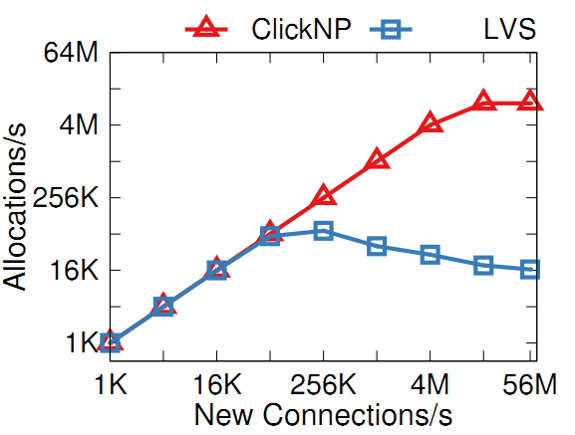
\includegraphics[width=4in]{l4alloc}
\caption{第4层负载均衡处理能力对比} \label{fig:l4alloc}
\note{包大小为64字节}
\end{figure}
